%%%%%%%%%%%%%%%%%%%%%%%%%%%%%%%%%%%%%%%%%
% Journal Article
% LaTeX Template
% Version 1.3 (9/9/13)
%
% This template has been downloaded from:
% http://www.LaTeXTemplates.com
%
% Original author:
% Frits Wenneker (http://www.howtotex.com)
%
% License:
% CC BY-NC-SA 3.0 (http://creativecommons.org/licenses/by-nc-sa/3.0/)
%
%%%%%%%%%%%%%%%%%%%%%%%%%%%%%%%%%%%%%%%%%
%----------------------------------------------------------------------------------------
%       PACKAGES AND OTHER DOCUMENT CONFIGURATIONS
%----------------------------------------------------------------------------------------
\documentclass[a4paper,11pt]{article}
%//TODO: pages have to be switched off before the ECB submission
%\pagenumbering{gobble}
\usepackage[english]{babel} % English language/hyphenation
\usepackage{amsmath,amsfonts,amsthm} % Math packages
\usepackage{nicefrac}
\usepackage[utf8]{inputenc}
\usepackage{float}
\usepackage{lipsum} % Package to generate dummy text throughout this template
\usepackage{blindtext}
\usepackage{graphicx} 
\usepackage{caption}
\newcommand{\source}[1]{\vspace{-10pt} \caption*{\footnotesize{\emph{Sources: }{#1}}}}
\newcommand{\desc}[1]{\vspace{-10pt} \caption*{\footnotesize{\emph{Notes: }{#1}}}}
\usepackage{subcaption}
\usepackage[sc]{mathpazo} % Use the Palatino font
\usepackage[T1]{fontenc} % Use 8-bit encoding that has 256 glyphs
\usepackage{setspace}
\setstretch{1.5}
\usepackage{microtype} % Slightly tweak font spacing for aesthetics
\usepackage[hmargin=2.5cm,vmargin=2.5cm]{geometry}
\usepackage{multicol} % Used for the two-column layout of the document
%\usepackage[hang, small,labelfont=bf,up,textfont=it,up]{caption} % Custom captions under/above floats in tables or figures
\usepackage{booktabs} % Horizontal rules in tables
\usepackage{float} % Required for tables and figures in the multi-column environment - they need to be placed in specific locations with the [H] (e.g. \begin{table}[H])
\usepackage{titletoc}
\usepackage[unicode=true,pdfusetitle,bookmarks=true,bookmarksnumbered=false,bookmarksopen=false,breaklinks=false,pdfborder={0 0 0},pdfborderstyle={},backref=false,colorlinks=true]{hyperref}
\hypersetup{urlcolor=blue, citecolor=blue, linkcolor=red}
\usepackage{lettrine} % The lettrine is the first enlarged letter at the beginning of the text
\usepackage{paralist} % Used for the compactitem environment which makes bullet points with less space between them
\usepackage{abstract} % Allows abstract customization
\renewcommand{\abstractnamefont}{\normalfont\bfseries} % Set the "Abstract" text to bold
\usepackage{titlesec} % Allows customization of titles
\usepackage{colortbl}
\definecolor{grey}{cmyk}{0, 0, 0, 0.17}
\usepackage{appendix} % For appendices
\usepackage{pgffor}    % For the loop
\usepackage{eurosym}
\usepackage{pdflscape} % Added package for landscape pages
\usepackage{array} % Added package to ensure landscape tables with fixed width
\usepackage{tikz}
\usetikzlibrary{positioning}


\titleformat{\section}[block]{\large\scshape\centering}{\thesection.}{1em}{} % Change the look of the section titles
\titleformat{\subsection}[block]{\large}{\thesubsection.}{1em}{} % Change the look of the section titles
\newcommand{\horrule}[1]{\rule{\linewidth}{#1}} % Create horizontal rule command with 1 argument of height
\usepackage{fancyhdr} % Headers and footers
\pagestyle{fancy} % All pages have headers and footers
\fancyhead{} % Blank out the default header
\fancyfoot{} % Blank out the default footer
\fancyhead[C]{} % Custom header text
\renewcommand{\headrulewidth}{0pt}

\fancyfoot[RO,LE]{\thepage} % Custom footer text
\usepackage{natbib}

% Define the path as a variable at the beginning of your document
\input{draftPaper_localBibliographyPath.tex}

%----------------------------------------------------------------------------------------
%       TITLE SECTION
%----------------------------------------------------------------------------------------
\title{\vspace{-15mm}\fontsize{20pt}{18pt}\selectfont\textbf{The EAGLE model with individual euro area countries: a framework for fiscal policy analysis}} % Article title
\author{
\large
{\textsc{Krzysztof~Ba\'nkowski\footnote{European Central Bank, Fiscal Policies Division - DG Economic Developements, Sonnemannstraße 20, 60314 Frankfurt am Main, E-Mail: krzysztof.bankowski@ecb.europa.eu}}}\\[2mm]
{\textsc{Emilė Petravičiūtė\footnote{European Central Bank, Fiscal Policies Division - DG Economic Developements, Sonnemannstraße 20, 60314 Frankfurt am Main, E-Mail: emile.petraviciute@ecb.europa.eu}}}\\[2mm]
%\thanks{A thank you or further information}\\ % Your name
%\normalsize \href{mailto:marco.torres.810@gmail.com}{marco.torres.810@gmail.com}\\[2mm] % Your email address
}
\date{\today}

%----------------------------------------------------------------------------------------
\begin{document}
\maketitle % Insert title

\begin{center}
    \textbf{\Large{Preliminary Draft}}
    
    \textit{This paper is a preliminary version and is currently under review. Please do not quote or cite without the author's permission.}
\end{center}

\begin{abstract}
    This paper presents an extension of the EAGLE (Euro Area and Global Economy) model that singles out 10 early-adopting euro area countries, enhancing the model’s capacity to analyze fiscal policy dynamics and cross-country spillovers. The extended framework incorporates meaningful fiscal policy channels, most notably, government consumption and investment, while carefully calibrating trade relationships using input-output tables to capture the heterogeneous import content across countries and demand components. Model simulations demonstrate that union-wide fiscal expansions generate significant multiplier effects, with government consumption showing stronger immediate impact than government investment. When applied to evaluate the Next Generation EU (NGEU) program, the model projects a peak increase in euro area GDP of 0.5\% relative to baseline, with effects persisting beyond the program's implementation period. The program's impact is concentrated in primary beneficiary countries like Spain and Italy as cross-border spillover effects through trade channels remain limited. The analysis highlights the model's utility in assessing complex policy initiatives within the Economic and Monetary Union while accounting for country-specific characteristics and interdependencies.

    \bigskip{}

    \noindent\textbf{Keywords:} EAGLE model, Fiscal policy, Euro area, Cross-country spillovers, Next Generation EU

    \bigskip{}

    \noindent\textbf{JEL Codes:} E62, F41, F42, F45

    \bigskip{}
    
    \clearpage{}
    
    \pagebreak{}    

\end{abstract}

\startcontents 
\printcontents{ }{1}{\section*{Table of content}}

\thispagestyle{fancy} % All pages have headers and footers

\section{Introduction and motivation}

% 1 Importance of heterogenity and interdependence
Interdependence and heterogeneity in the euro area are central to understanding the region's macroeconomic dynamics, given its unique institutional framework, where a common monetary policy operates alongside decentralized fiscal and structural policies. Interdependence arises primarily through strong trade linkages and the transmission of monetary policy, implying that shocks in one member state—such as fiscal adjustments—can propagate across the union, amplifying volatility and influencing policy effectiveness. At the same time, persistent heterogeneity, reflected in disparities in productivity, debt dynamics, and structural rigidities, stems from differentiated policy priorities, institutional legacies, and varying degrees of economic resilience. These asymmetries pose challenges for union-wide stabilization efforts and risk exacerbating economic fragmentation. A comprehensive understanding of both interdependence and heterogeneity within the Economic and Monetary Union (EMU) is therefore essential for designing policies that mitigate fragmentation risks, enhance shock absorption, and reconcile national policy autonomy with collective stability. In this context, the development of analytical tools to improve euro area-wide institutions' capacity—such as the European Central Bank (ECB)—to assess and address these dynamics is of critical importance.

\begin{figure}[H]
    \centering
    \caption{The magnitude of imports across euro area countries, compared to Japan and the US. \label{fig1}}
    \includegraphics[width=150mm]{figures/importMagnitude.png}
    \vspace{5mm} \source{World Integrated Trade Solution Database of the World Bank, 2022 data.}
    % \\TODO: check the data source
    %\desc{The fiscal shock is based on a comparable increase in government purchases in both regions, representing an ex-ante 1\% of GDP fiscal expansion at the union level.}
\end{figure}

% 2 We establish a more granular version of EAGLE with 11 original member states
A key macroeconomic framework employed within the Eurosystem to analyze both interdependence and heterogeneity in the EMU has been the EAGLE model, developed in the 2010s (\citet{Gomesaetal2012}). This multi-country extension of the seminal New Area-Wide Model initially represented the euro area as a two-region economy—Germany and the rest of the euro area—alongside the United States and the rest of the world. While EAGLE has proven valuable for assessing economic policies within a multi-country setting, its structure limits its ability to evaluate large-scale initiatives such as the Next Generation EU (NGEU) program, which involves complex cross-country interactions. Moreover, the model abstracts from the role of individual euro area economies (except for Germany), despite their significant contributions to the union's aggregate dynamics. 

To address these limitations, we extend the EAGLE framework by distinguishing 10 early euro-adopting countries—Austria, Belgium, Finland, France, Germany, Greece, Italy, the Netherlands, Portugal, and Spain. In addition, we explicitly single out the rest of the European Union (i.e., EU countries outside the euro area), given its strong economic ties with the Eurozone. This extension enhances the model's ability to capture country-specific dynamics and provides a more granular representation of economic interdependencies within the EMU.

% 4 This is just moved from the model section (see whether it fits when working on the introduction)
A crucial aspect to be incorporated into our model extension is the significant role of trade in interconnecting the euro area and linking it to the global economy. The euro area is characterized by deep regional integration, facilitated by the single currency and the European Single Market. Intra-euro area trade constitutes a substantial share of member states' total trade flows, with Germany often serving as a central node, both as a major exporter and importer. At the same time, the euro area maintains a strong trade presence globally, ranking among the world's largest trading blocs. Its openness to trade, with total trade exceeding 30\% of GDP, underscores its importance as a global trading hub. When measured by the import-to-GDP ratio, euro area economies exhibit significantly higher openness compared to other major advanced economies, such as Japan and the United States (see Figure \ref{fig1}). Additionally, the euro area has historically maintained on aggregate sizable trade surpluses, largely driven by its strong manufacturing sector. These trade dynamics are critical for understanding macroeconomic shock transmission within the euro area and beyond, and we aim to incorporate these features comprehensively in our extended model.

\section{The model}

\subsection{The model extension}

% (1)
The EAGLE model portrays the global economy as composed of multiple countries/regions, some of which form a monetary union. The original version, initially introduced in \citet{Gomesaetal2010ecbwp} and later published in \citet{Gomesaetal2012}, included Germany, the rest of the euro area, the United States, and the rest of the world. Subsequent versions of the model have modified the country composition to focus on different economic contexts, such as small open economies like Ireland and Slovenia (\citealp{Clancyetal2016}), the four largest euro area economies—Germany, France, Italy, and Spain (\citealp{BokanEtAl2018em})—or non-euro area countries like Hungary (\citealp{BekesiEtAl2017mnbwp}). Regardless of the specific configuration, regions within the EAGLE framework are modeled as open economies, interconnected through bilateral trade relationships and a common monetary policy for euro area members.

% (2)
% \\TODO: for Emile, check the numbers on the EA shares
% \\TODO: having a chart with the GDP shares could be nice here
Our version of the EAGLE model advances the representation of the euro area by disaggregating it into ten member states—Austria, Belgium, Finland, France, Germany, Greece, Italy, the Netherlands, Portugal, and Spain—which together account for approximately 95\% of the EMU's GDP, alongside a residual bloc representing the remaining 5\%. In addition to the United States, we distinguish the non-euro area EU region, reflecting its close economic ties with the euro area. Overall, our version of EAGLE comprises 14 countries or regions, constituting, to the best of our knowledge, the most extensive extension of the model to date in terms of country disaggregation.

% (3)
The EAGLE model has been extensively employed to analyze a wide range of economic policy issues, including global fiscal stimulus (\citealp{GomesEtAl2015jimf}), structural reforms (\citealp{Gomesetal2013if}; \citealp{Jacquinot2018springer}; \citealp{Gomes2018jm}), monetary union accession (\citealp{BrzozaBrzezinaEtAl2014oer}), fiscal devaluations (\citealp{GomesEtAl2016em}), trade tariffs and protectionism (\citealp{BoltEtAl2019dnbwp}; \citealp{JacquinotEtAl2022jimf}; \citealp{ClancyEtAl2024ijcb}), financial interlinkages (\citealp{Pariesetal2016ecbwp}; \citealp{BokanEtAl2018em}), and economic risks associated with high government debt (\citealp{BurielEtAl2020ecbwp}). This paper applies the extended version of the EAGLE model to assess the macroeconomic impact of the recently launched multi-year EU-wide investment initiative—Next Generation EU (NGEU). In doing so, it complements existing analyses involving the EAGLE framework (\citealp{Bankowskietal2021ecbOP}; \citealp{Bankowskietal2022ecbOP}; \citealp{Bankowskietal2025ecbOP}) by leveraging the detailed country disaggregation. This enhanced structure enables the assessment of the program's effects on smaller member states, such as Greece and Portugal, which are among the major beneficiaries of the NGEU.

% (4)
As in other large-scale DSGE models, our version incorporates a share of non-Ricardian households and features several real and nominal rigidities, including habit formation, adjustment costs for investment and imports, and Calvo-type pricing of intermediate goods and wage setting with partial indexation. In this subsection, we limit the description of the model to those elements that are crucial for our extension and policy application, with particular focus on the bundling of final goods, trade specification, and policy rules. For all other aspects, we refer the reader to \citet{Gomesaetal2012} for the general model characteristics and to \citet{Clancyetal2016} for the enhanced fiscal policy specification.

% (6)
\paragraph{Final good production.} 

Our model distinguishes four types of final goods: private consumption, private investment, government consumption, and government investment. Each type of good is assembled by firms operating under perfect competition. At the origin of the process, the inputs for assembly are intermediate goods produced by firms under monopolistic competition in two sectors—non-tradable (akin to services) and tradable (akin to manufacturing). Tradable goods are also subject to international trade. Consequently, goods purchased by the government may contain imported components, with the extent of import content determined by a home-bias parameter. Although all final goods ultimately originate from the intermediate tradable and non-tradable sectors, the assembly processes are independent across categories. In practice, this implies, for example, that the import content of government consumption differs from that of private consumption, reflecting the tendency of governments to purchase domestically produced goods. Further details on the calibration of these parameters are provided in Subsection~\ref{sec:model_calibration}, with the specification of the multi-country trade structure constituting a major contribution of this paper.

Specifically, each of the four types of goods $Q_t^i$ is assembled using a constant elasticity of substitution (CES) technology (see Eq.~\ref{eq1}), combining tradable goods $TT_t^i$ and domestically produced non-tradable goods $NT_t^i$. The parameter $v_i$ governs the share of each input in the bundle, while $\mu_i$ denotes the elasticity of substitution between them:
\begin{equation}
    \label{eq1}
    Q_t^i = \left[v_i^{\frac{1}{\mu_i}}\left(TT_t^i\right)^{\frac{\mu_i-1}{\mu_i}} + \left(1-v_i\right)^{\frac{1}{\mu_i}}\left(NT_t^i\right)^{\frac{\mu_i-1}{\mu_i}}\right]^{\frac{\mu_i}{\mu_i-1}}.
\end{equation}
The tradable good $TT_t^i$, in turn, is produced analogously as a CES composite of home-produced tradable goods $HT_t^i$ and imported goods $IM_t^i$ (see Eq.~\ref{eqTT}). The parameter $v_{Ti}$ captures the home bias in tradable goods, and $\mu_{Ti}$ measures the elasticity of substitution between domestic and imported goods:
\begin{equation}
    \label{eqTT}
    TT_t^i = \left[v_{Ti}^{\frac{1}{\mu_{Ti}}}\left(HT_t^i\right)^{\frac{\mu_{Ti}-1}{\mu_{Ti}}} + \left(1-v_{Ti}\right)^{\frac{1}{\mu_{Ti}}}\left(IM_t^i\right)^{\frac{\mu_{Ti}-1}{\mu_{Ti}}}\right]^{\frac{\mu_{Ti}}{\mu_{Ti}-1}}.
\end{equation}
Finally, the imported good $IM_t^i$ consists of a bundle of bilateral imports $IM_t^{i,CO}$ (see Eq.~\ref{eqIM}). The parameter $v_{Mi}^{H,CO}$ represents the share of imports from country or region $CO$, satisfying $\sum_{CO \neq H} v_{Mi}^{H,CO} = 1$, and $\mu_{Mi}$ is the elasticity of substitution between imports from different trading partners:
\footnote{The country-specific import weights $v_{Mi}^{H,CO}$ are determined as a function of the relative economic size and the degree of openness. Accordingly, even if Germany exhibits the same degree of openness to imports from Austria and France, the weight $v_{Mi}^{DE,AT}$ is expected to be significantly smaller than $v_{Mi}^{DE,FR}$, reflecting the larger size of the French economy.}
\begin{equation}
    \label{eqIM}
    IM_t^i = \left[\sum_{CO \neq H} \left(v_{Mi}^{H,CO}\right)^{\frac{1}{\mu_{Mi}}} \left(IM_t^{i,CO}\right)^{\frac{\mu_{Mi}-1}{\mu_{Mi}}}\right]^{\frac{\mu_{Mi}}{\mu_{Mi}-1}}.
\end{equation}
Figure~\ref{finalGoodProduction} offers a detailed schematic representation of the production of a final good of type $i$.
\footnote{The CES aggregation framework also implies that the prices of final goods are composite indices of the prices of their underlying components. Specifically, the price of a final good of type $i$, denoted $P_{i,t}$, the price of the tradable component $P_{TTi,t}$, and the price of imported tradable goods $P_{IMi,t}$ are defined as follows: 
\[
P_{i,t} = \left[v_i\left(P_{TTi,t}\right)^{1-\mu_i} + \left(1-v_i\right)\left(P_{NT,t}\right)^{1-\mu_i}\right]^{\frac{1}{1-\mu_i}},
\]
\[
P_{TTi,t} = \left[v_{Ti}\left(P_{HT,t}\right)^{1-\mu_{Ti}} + \left(1-v_{Ti}\right)\left(P_{IMi,t}\right)^{1-\mu_{Ti}}\right]^{\frac{1}{1-\mu_{Ti}}},
\]
\[
P_{IMi,t} = \left[\sum_{CO \neq H} v_{Mi}^{H,CO}\left(P_{IM,t}^{CO}\right)^{1-\mu_{Mi}}\right]^{\frac{1}{1-\mu_{Mi}}}.
\]
Here, $v_i$, $v_{Ti}$, and $v_{Mi}^{H,CO}$ are the share parameters governing the aggregation at each respective level, and $\mu_i$, $\mu_{Ti}$, and $\mu_{Mi}$ denote the elasticities of substitution. The price $P_{NT,t}$ corresponds to domestically produced non-tradable goods, $P_{HT,t}$ denotes the price of home-produced tradable goods, and $P_{IM,t}^{CO}$ refers to the price of imports from country or region $CO$. The structure of price aggregation mirrors the quantity aggregation.}

\begin{figure}[H]
    \centering
    \caption{Production of final goods in the EAGLE model.
    \label{finalGoodProduction}}
    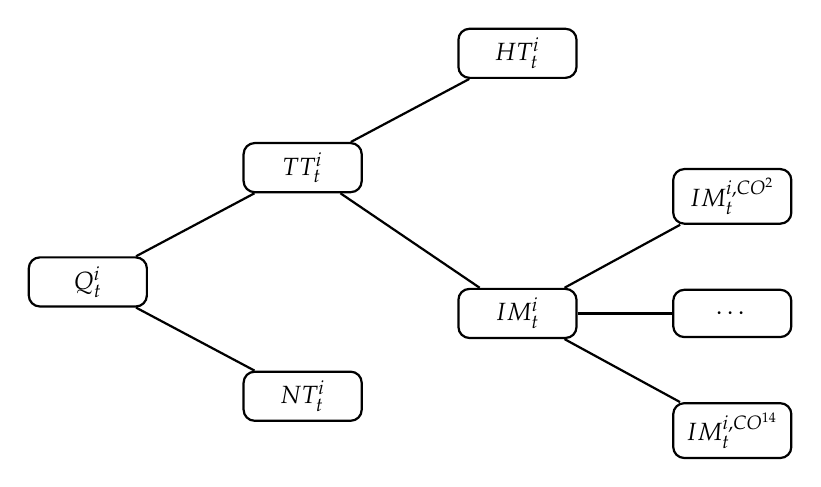
\begin{tikzpicture}[
        node distance=0.8cm and 1.2cm, % tighter horizontal and vertical distances
        every node/.style={draw, rounded corners, minimum width=1.5cm, minimum height=0.6cm, align=center, font=\small},
        every path/.style={draw, thick} % thick lines, no arrows
      ]
      
      % Nodes
      \node (qt) {$Q_t^i$};
      \node[above right=of qt] (tt) {$TT_t^i$};
      \node[below right=of qt] (nt) {$NT_t^i$};
      \node[above right=of tt] (ht) {$HT_t^i$};
      \node[below right=of tt, yshift=-0.4cm] (im) {$IM_t^i$};
      \node[above right=of im] (im_CO1) {$IM_t^{i,CO^2}$};
      \node[right=of im] (im_CO2) {$\dots$};
      \node[below right=of im] (im_CO3) {$IM_t^{i,CO^{14}}$};
    
      % Edges
      \draw (qt) -- (tt);
      \draw (qt) -- (nt);
      \draw (tt) -- (ht);
      \draw (tt) -- (im);
      \draw (im) -- (im_CO1);
      \draw (im) -- (im_CO2);
      \draw (im) -- (im_CO3);
    
    \end{tikzpicture}
    
    \vspace{5mm}
    \small
    \begin{minipage}{0.9\textwidth}
    \textit{Notes}: $Q_t^i$ denotes the final good of type $i$; $TT_t^i$ is the tradable component used in the bundling of good $i$; $NT_t^i$ is the non-tradable component; $HT_t^i$ represents the home-produced tradable good; $IM_t^i$ denotes the imported tradable good; $IM_t^{i,CO^2}$ and $IM_t^{i,CO^{14}}$ represent imports from countries $CO^2$ and $CO^{14}$, respectively, used in the production of good $i$.
    \end{minipage}
\end{figure}

\paragraph{Resource constraint} Countries or regions in the EAGLE model are subject to the following aggregate resource constraint, which can be expressed in nominal terms as shown in Eq.~\ref{eqResourceConstraint}. Total production $Y_t$ is allocated to satisfy the domestic share of final demand from the private sector ($C_t$ and $I_t$) and the general government ($G_{C,t}$ and $G_{I,t}$), as well as to meet external demand through exports.\footnote{Some of the production is absorbed by transaction costs and capital utilization costs, represented by $\Gamma_{v,t}$ and $\Gamma_u(u_t)K_t$, respectively.} Figure~\ref{figAggResourceConstraint} provides a schematic representation of the creation and utilization of resources within a country or region in the EAGLE model.
\begin{equation} \label{eqResourceConstraint}
    \begin{aligned}
        P_{Y,t} Y_t =\ & P_{C,t} \underbrace{\left(C_t + \Gamma_{v,t}\right)}_{Q_t^{C}} + P_{I,t} \underbrace{\left(I_t + \Gamma_u(u_t) K_t\right)}_{Q_t^{I}} + P_{G_C,t} \underbrace{G_{C,t}}_{Q_t^{G_c}} + P_{G_I,t} \underbrace{G_{I,t}}_{Q_t^{G_i}} \\
        & + \sum_{CO \neq H} \frac{s^{CO}}{s^H} S_t^{H,CO} P_{X,t}^{H,CO} IM_t^{CO,H} - \sum_{CO \neq H} P_{IM,t}^{H,CO} IM_t^{H,CO}.
    \end{aligned}
\end{equation}

%// NOTE: In the budget constraint the equations refer to Qs variables, which include adjustment costs.

\begin{figure}[H]
    \centering
    \caption{Production and utilization of resources within a country or region in the EAGLE model.
    \label{figAggResourceConstraint}}
    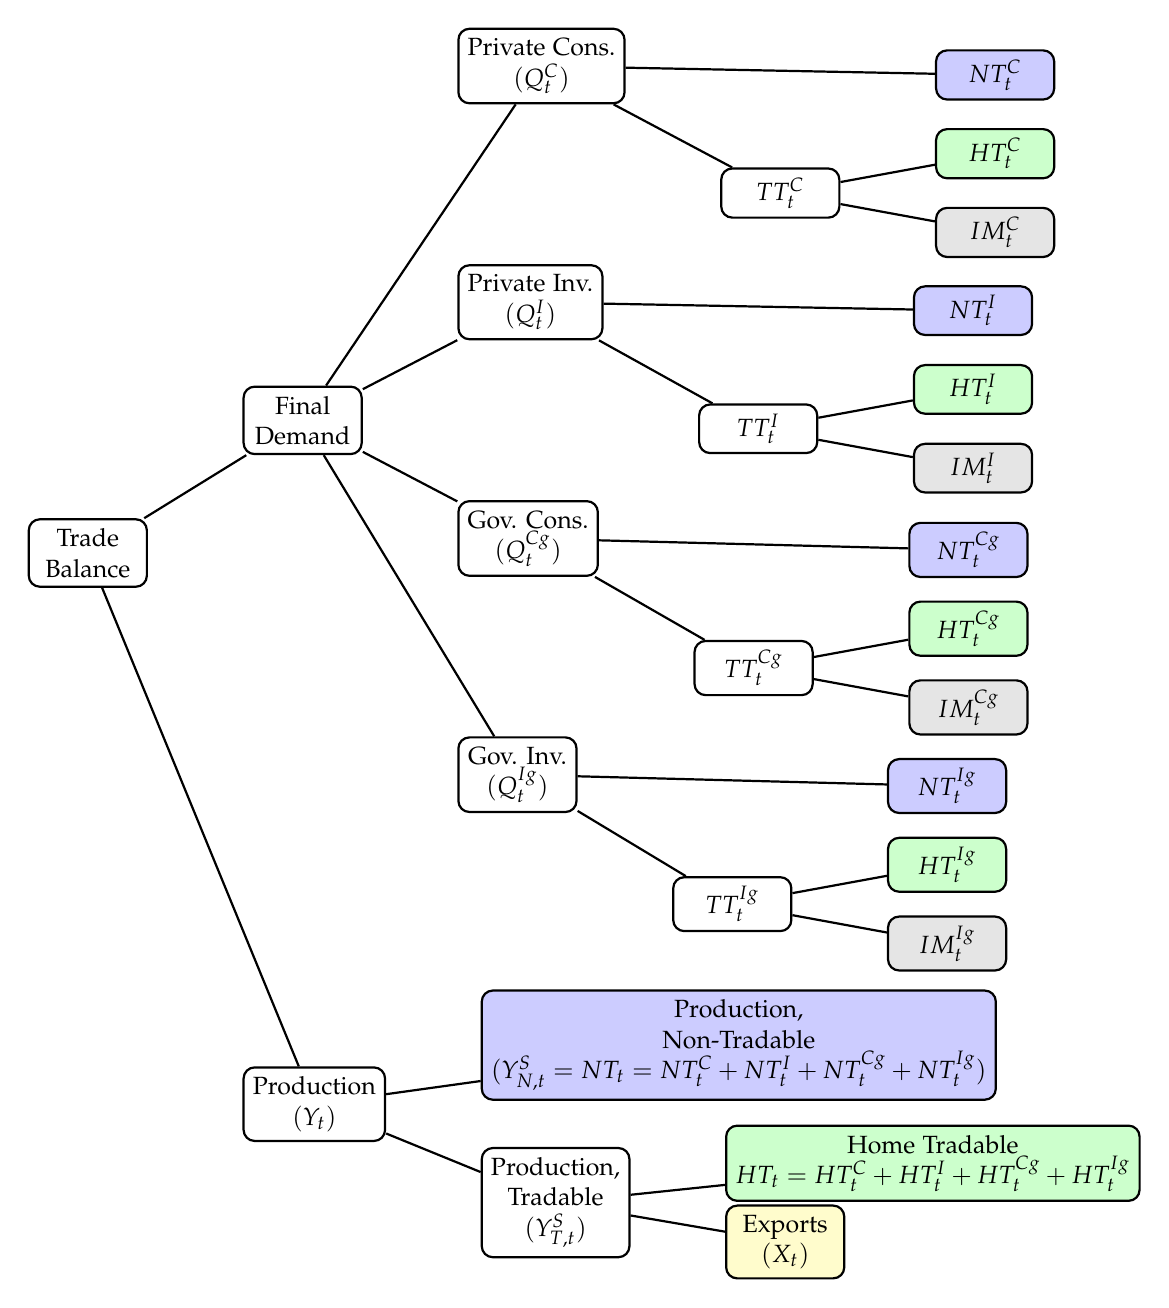
\begin{tikzpicture}[
        node distance=0.8cm and 1.2cm, % tighter horizontal and vertical distances
        every node/.style={draw, rounded corners, minimum width=1.5cm, minimum height=0.6cm, align=center, font=\small},
        every path/.style={draw, thick} % thick lines, no arrows
    ]
    
    % Nodes
    \node (tb) {Trade\\ Balance};
    \node[above right=of tb] (demand) {Final\\ Demand};
    \node[right=of tb, yshift=-7cm] (y) {Production\\ $(Y_t)$};
    
    \node[right=of demand, yshift=4.5cm] (qc) {Private Cons.\\ $(Q_t^C)$};
    \node[right=of demand, yshift=1.5cm] (qi) {Private Inv.\\ $(Q_t^I)$};
    \node[right=of demand, yshift=-1.5cm] (qcg) {Gov. Cons.\\ $(Q_t^{Cg})$};
    \node[right=of demand, yshift=-4.5cm] (qig) {Gov. Inv.\\ $(Q_t^{Ig})$};
    
    \node[below right=of qc] (ttc) {$TT_t^C$};
    \node[below right=of qi] (tti) {$TT_t^I$};
    \node[below right=of qcg] (ttcg) {$TT_t^{Cg}$};
    \node[below right=of qig] (ttig) {$TT_t^{Ig}$};
    
    \node[right=of ttc, yshift=1.5cm, fill=blue!20] (ntc) {$NT_t^C$};
    \node[right=of tti, yshift=1.5cm, fill=blue!20] (nti) {$NT_t^I$};
    \node[right=of ttcg, yshift=1.5cm, fill=blue!20] (ntcg) {$NT_t^{Cg}$};
    \node[right=of ttig, yshift=1.5cm, fill=blue!20] (ntig) {$NT_t^{Ig}$};
    
    \node[right=of ttc, yshift=0.5cm, fill=green!20] (htc) {$HT_t^C$};
    \node[right=of tti, yshift=0.5cm, fill=green!20] (hti) {$HT_t^I$};
    \node[right=of ttcg, yshift=0.5cm, fill=green!20] (htcg) {$HT_t^{Cg}$};
    \node[right=of ttig, yshift=0.5cm, fill=green!20] (htig) {$HT_t^{Ig}$};
    
    \node[right=of ttc, yshift=-0.5cm, fill=gray!20] (imc) {$IM_t^C$};
    \node[right=of tti, yshift=-0.5cm, fill=gray!20] (imi) {$IM_t^I$};
    \node[right=of ttcg, yshift=-0.5cm, fill=gray!20] (imcg) {$IM_t^{Cg}$};
    \node[right=of ttig, yshift=-0.5cm, fill=gray!20] (imig) {$IM_t^{Ig}$};
    
    \node[right=of y, yshift=0.75cm, fill=blue!20] (ysn) {Production,\\ Non-Tradable\\ $(Y_{N,t}^S = NT_t = NT_t^C + NT_t^I + NT_t^{Cg} + NT_t^{Ig})$};
    \node[right=of y, yshift=-1.25cm] (yst) {Production,\\ Tradable\\ $(Y_{T,t}^S)$};
    
    \node[right=of yst, yshift=0.5cm, fill=green!20] (nt) {Home Tradable\\ $HT_t = HT_t^C + HT_t^I + HT_t^{Cg} + HT_t^{Ig}$};
    \node[right=of yst, yshift=-0.5cm, fill=yellow!20] (xt) {Exports\\ $(X_t)$};
    
    % Edges
    \draw (tb) -- (demand);
    \draw (tb) -- (y);
    
    \draw (demand) -- (qc);
    \draw (demand) -- (qi);
    \draw (demand) -- (qcg);
    \draw (demand) -- (qig);
    
    \draw (qc) -- (ttc);
    \draw (qi) -- (tti);
    \draw (qcg) -- (ttcg);
    \draw (qig) -- (ttig);
    
    \draw (qc) -- (ntc);
    \draw (qi) -- (nti);
    \draw (qcg) -- (ntcg);
    \draw (qig) -- (ntig);
    
    \draw (ttc) -- (htc);
    \draw (tti) -- (hti);
    \draw (ttcg) -- (htcg);
    \draw (ttig) -- (htig);
    
    \draw (ttc) -- (imc);
    \draw (tti) -- (imi);
    \draw (ttcg) -- (imcg);
    \draw (ttig) -- (imig);
    
    \draw (y) -- (ysn);
    \draw (y) -- (yst);
    
    \draw (yst) -- (nt);
    \draw (yst) -- (xt);
    
    \end{tikzpicture}
        
    \vspace{5mm}
    \small
    \begin{minipage}{0.9\textwidth}
        \textit{Notes}: $TT_t^i$ denotes the tradable good for each type of good $i$, where $i \in \{C, I, Cg, Ig\}$. Analogously, $NT_t^i$, $HT_t^i$, and $IM_t^i$ represent, respectively, the non-tradable good, the home tradable good, and imported goods for the various sectors. Since the production of non-tradables and home tradable goods is used to meet final demand domestically, any trade imbalance arises from the difference between imports and the production allocated to exports (indicated by the grey and yellow nodes).

    \end{minipage}
\end{figure}

\paragraph{Trade and net foreign asses position} Each country or region in the EAGLE model may experience a mismatch between the value of imported and exported goods, resulting in a trade surplus or deficit. The trade balance in nominal terms is defined as the difference between exports and imports (see Eq.~\ref{eqTradeBalance}):
\footnote{$S_t^{H,CO}$ in Eq.~\ref{eqTradeBalance} denotes the nominal exchange rate that converts the price $P_{X,t}^{H,CO}$, expressed in the currency of country $CO$, into the currency of country $H$.}
\begin{equation} \label{eqTradeBalance}
    TB_t \equiv \sum_{CO \neq H} S_t^{H,CO} P_{X,t}^{H,CO} \underbrace{\frac{s^{CO}}{s^H} IM_t^{CO,H}}_{\equiv X_t^{H,CO}} - \sum_{CO \neq H} P_{IM,t}^{H,CO} IM_t^{H,CO}.
\end{equation}
From Eq.~\ref{eqTradeBalance}, it follows that exports from country $H$ to country $CO$ ($X_t^{H,CO}$) correspond to the imports of country $CO$ from $H$, adjusted by the ratio of their economic sizes $\left(\frac{s^{CO}}{s^H}\right)$. If country $CO$ is significantly larger than country $H$, even minor changes in its bilateral imports from $H$ can generate substantial fluctuations in $H$'s exports. This feature presents a major challenge for calibrating and solving the steady state of the model when incorporating countries of vastly different sizes (see Section~\ref{sec:model_calibration} for further discussion).

Trade imbalances between countries are reflected in their net foreign asset (NFA) positions, which materialize through international bond holdings. In the model, internationally traded bonds are denominated in the currency of the core country—the United States—and thus in U.S. dollars. Under this setup, a country's NFA position evolves according to Eq.~\ref{eqNetForeignAssetPosition}:
\begin{equation} \label{eqNetForeignAssetPosition}
    R_t^{*-1} B_{t+1}^* = B_t^* + \frac{TB_t^{\mathrm{CO}}}{S_t^{\mathrm{CO},\mathrm{US}}},
\end{equation}
where $R_t^*$ denotes the gross return on the internationally traded bond $B_{t+1}^*$, and $S_t^{\mathrm{CO},\mathrm{US}}$ represents the nominal exchange rate, defined as the price of one U.S. dollar in terms of the currency of country or region $\mathrm{CO}$. Finally, the assumption of zero net supply of international bonds implies the global market clearing condition $\sum_{\mathrm{CO}} s^{\mathrm{CO}} B_t^{*\mathrm{CO}} = 0$, with $\sum_{\mathrm{CO}} s^{\mathrm{CO}} = 1$.

\paragraph{Euro area aggregation} As the euro area is composed of ten individual countries and a residual region, each modeled as an open economy, it is necessary to construct aggregate indicators for the monetary union. In particular, aggregation is required for euro area-wide output $(Y_t^{EA})$ and inflation $(\Pi_t^{EA,4})$, as defined in Equations~\ref{eqEAoutput} and~\ref{eqEAinflation}, respectively. The set of countries and the residual region constituting the euro area is denoted by \(\mathcal{I}^{EA} = \{ \text{AT}, \text{BE}, \text{FI}, \text{FR}, \text{DE}, \text{GR}, \text{IT}, \text{NL}, \text{PT}, \text{ES}, \text{RA} \}\), where \(s^i\) represents the relative size of country or region \(i\).

\begin{equation} \label{eqEAoutput}
    Y_t^{EA} \equiv \frac{\sum\limits_{i \in \mathcal{I}^{EA}} s^i \overline{P_Y^{i}} Y_t^i}{\sum\limits_{i \in \mathcal{I}^{EA}} s^i},
\end{equation}
\begin{equation} \label{eqEAinflation}
    \Pi_t^{EA,4} \equiv \prod\limits_{i \in \mathcal{I}^{EA}} \left( \frac{P_{C,t}^i}{P_{C,t-4}^i} \right)^{\frac{s^i}{\sum\limits_{i \in \mathcal{I}^{EA}} s^i}}.
\end{equation}

\paragraph{Fiscal and monetary policy rules} Regarding the general government specification, the budget encompasses multiple tax and expenditure instruments. With the possibility to issue bonds, governments are not required to balance the budget in each period. Following the extension by \citet{Clancyetal2016}, both government consumption and investment play a meaningful role in the model. Specifically, government consumption exhibits complementarity with private consumption, while government investment contributes to the stock of productive capital, thereby enhancing the production capacity of the private sector.
\footnote{The complementarity between government and private consumption is introduced through the specification of a composite good consumed by households, following the approach of \citet{Coenen-et-al_AER_2012}. Specifically, the composite consumption good $\tilde{C}_t$ is modeled as a CES aggregate of final private consumption and final government consumption goods: $\tilde{C}_t = \left[v_{\text{CCES}}^{\frac{1}{\mu_{\text{CCES}}}}\left(C_t\right)^{\frac{\mu_{\text{CCES}}-1}{\mu_{\text{CCES}}}} + \left(1-v_{\text{CCES}}\right)^{\frac{1}{\mu_{\text{CCES}}}}\left(G_{C,t}\right)^{\frac{\mu_{\text{CCES}}-1}{\mu_{\text{CCES}}}}\right]^{\frac{\mu_{\text{CCES}}}{\mu_{\text{CCES}}-1}}$,where $v_{\text{CCES}}$ denotes the share parameter, and $\mu_{\text{CCES}}$ represents the elasticity of substitution between the two component goods.}
\footnote{The assumption that government investment enhances productivity builds on the work of \citet{LeeperEtAl2010jme}, where public capital accumulation is governed by $K_{G,t+1} = (1-\delta_G)K_{G,t} + G_{I,t}$. This formulation implies that government investment $G_{I,t}$ builds up the stock of public capital $K_{G,t+1}$, which depreciates at the rate $\delta_G$. Public capital, in turn, enters the production function of both tradable and non-tradable goods, specified respectively as $Y_{T,t}^S = z_{T,t} K_{G,t}^{\alpha_G} (K_{T,t}^D)^{\alpha_T} (N_{T,t}^D)^{1-\alpha_T} - \psi_T$ and $Y_{N,t}^S = z_{N,t} K_{G,t}^{\alpha_G} (K_{N,t}^D)^{\alpha_N} (N_{N,t}^D)^{1-\alpha_N} - \psi_N$, thereby enhancing the productive capacity of the private sector. Here, $Y_{T,t}^S$ and $Y_{N,t}^S$ denote sectoral outputs, $z_{T,t}$ and $z_{N,t}$ represent sector-specific productivity levels, $\alpha_G$ measures the contribution of public capital to production, $K_{T,t}^D$ and $K_{N,t}^D$ are private capital inputs, $N_{T,t}^D$ and $N_{N,t}^D$ are labor inputs, $\alpha_T$ and $\alpha_N$ denote the capital shares in the tradable and non-tradable sectors, respectively, and $\psi_T$ and $\psi_N$ capture fixed costs.}

%//NOTE: here is the decomposed budget constraint of the government > based on that we have 10 fisccal instruments
% (1) DE_pcg(-1)*DE_cg(-1)
% (2) +DE_pig(-1)*DE_ig(-1)
% (3) +DE_tr(-1)
% ( ) +DE_b(-1)*DE_pic(-1)^(-1)
% ( ) +DE_m(-2)*DE_pic(-1)^(-1) 
% (4) = DE_tauc(-1)*DE_c(-1)
% (5 & 6) +(DE_taun(-1)+DE_tauwh(-1))*(DE_wi(-1)*DE_ndi(-1)+DE_wj(-1)*DE_ndj(-1))
% (7) +DE_tauwf(-1)*DE_w(-1)*DE_nd(-1)
% (8) +DE_tauk(-1)*(DE_rk(-1)*DE_u(-1)-(DE_gammau(-1)+DE_delta)*DE_pi(-1))*DE_k(-1)
% (9) +DE_taud(-1)*DE_d(-1)
% (10) +DE_t(-1)
% ( ) +(DE_r(-1)*(1-DE_gammab(-1)))^(-1)*DE_b
% ( ) +DE_m(-1);

%//NOTE: let's see how each of these instruments is modelled
% (1): DE_pcg*DE_cg = DE_cgy*DE_pybar*DE_ybar; > DE_cgy = (1-DE_rhocg)*DE_cgybar+DE_rhocg*DE_cgy(-1)+DE_epsgc;
% (2): DE_pig*DE_ig = DE_igy*DE_pybar*DE_ybar; > DE_igy = (1-DE_rhoig)*DE_igybar+DE_rhoig*DE_igy(-1)+DE_epsgi;
% (3) DE_tr = DE_try*DE_pybar*DE_ybar; DE_try = (1-DE_rhotr)*DE_trybar+DE_rhotr*DE_try(-1)+DE_epstr;
% (4) DE_tauc = (1-DE_rhotauc)*DE_taucbar+DE_rhotauc*DE_tauc(-1)+DE_epstauc;
% (5) DE_taun = (1-DE_rhotaun)*DE_taunbar+DE_rhotaun*DE_taun(-1)+DE_epstaun;
% (6) DE_tauwh = (1-DE_rhotauwh)*DE_tauwhbar+DE_rhotauwh*DE_tauwh(-1)+DE_epstauwh;
% (7) DE_tauwf = (1-DE_rhotauwf)*DE_tauwfbar+DE_rhotauwf*DE_tauwf(-1)+DE_epstauwf;
% (8) DE_tauk = (1-DE_rhotauk)*DE_taukbar+DE_rhotauk*DE_tauk(-1)+DE_epstauk;
% (9) DE_taud = (1-DE_rhotaud)*DE_taudbar+DE_rhotaud*DE_taud(-1)+DE_epstaud;
% (10) DE_ty = DE_t/(DE_pybar*DE_ybar); > DE_t/(DE_pybar*DE_ybar) = DE_phitb*(DE_b/(DE_pybar*DE_ybar)-DE_bytarget);

In our version of the EAGLE model, the government is equipped with ten fiscal instruments. Seven of these operate on the revenue side of the budget: the consumption tax rate, $\tau_t^C$; the wage tax rate, $\tau_t^N$; the social contribution rate paid by employees, $\tau_t^{Wh}$; the social contribution rate paid by employers, $\tau_t^{Wf}$; the tax rate on capital returns, $\tau_t^k$; the tax rate on bond returns, $\tau_t^b$; and lump-sum taxes, $T_t$. The remaining three instruments are on the expenditure side of the budget: government consumption, $G_{C,t}$; government investment, $G_{I,t}$; and government transfers, $TR_t$.

For all fiscal instruments except for lump-sum taxes, we assume a fiscal rule of the following form:
\begin{equation}
    \label{eqFiscalRule}
    X_t = (1-\rho_X) \bar{X} + \rho_X X_{t-1} + \varepsilon_{X,t},
\end{equation}
where \(X \in \left\{ \tau_t^C, \tau_t^N, \tau_t^{Wh}, \tau_t^{Wf}, \tau_t^k, \tau_t^b, \frac{P_{G_C,t} G_{C,t}}{\overline{P_Y Y}}, \frac{P_{G_I,t} G_{I,t}}{\overline{P_Y Y}}, \frac{TR_t}{\overline{P_Y Y}} \right\}\). For expenditure instruments, the fiscal rule in Eq.~\ref{eqFiscalRule} operates on nominal ratios relative to steady-state nominal GDP. Here, $\bar{X}$ denotes the long-run target for the fiscal instrument, $\rho_X$ is the smoothing parameter, and $\varepsilon_{X,t}$ represents an i.i.d. fiscal shock specific to the instrument.

The fiscal rule governing lump-sum taxes is designed to ensure that government debt converges towards a long-run target level, $\overline{B_Y}$, which is calibrated. Stability of the debt stock is achieved through a gradual adjustment of lump-sum taxes relative to output, with the speed of adjustment governed by the parameter $\phi_{B_Y}$, as specified in Eq.~\ref{eqDebtRule}:
\begin{equation}
    \label{eqDebtRule}
    \frac{T_t}{\overline{P_Y Y}} = \phi_{B_Y} \left( \frac{B_t}{\overline{P_Y Y}} - \overline{B_Y} \right).
\end{equation}

%//NOTE: Let's talk about the monetary policy now.
% Here are the rules for the US.
% (for the US) 
% US_r^4-1 = US_phirr*(US_r(-1)^4-1)+(1-US_phirr)*(US_rrstar^4*US_pi4target-1+US_phirpi*(US_pic4-US_pi4target))+US_phirgy*(US_y/US_y(-1)-1)+US_epsr;
% (for the rest of the EU) 
% RU_r^4-1 = RU_phirr*(RU_r(-1)^4-1)+(1-RU_phirr)*(RU_rrstar^4*RU_pi4target-1+RU_phirpi*(RU_pic4-RU_pi4target))+RU_phirgy*(RU_y/RU_y(-1)-1)+RU_epsr;
% (for the rest of the world) 
% RW_r^4-1 = RW_phirr*(RW_r(-1)^4-1)+(1-RW_phirr)*(RW_rrstar^4*RW_pi4target-1+RW_phirpi*(RW_pic4-RW_pi4target))+RW_phirgy*(RW_y/RW_y(-1)-1)+RW_epsr;
% (for the EA) 
% DE_r^4-1 = EA_phirr*(DE_r(-1)^4-1)+(1-EA_phirr)*(DE_rrstar^4*DE_pi4target-1+EA_phirpi*(EA_pic4-DE_pi4target))	+EA_phirgy*(EA_ygrowth-1)+EA_epsr;
% The above rules fortunately coincide with what is in the EM paper.

Monetary authorities in the model conduct policy according to a Taylor-type interest rate rule, specified in terms of annual CPI inflation, $\Pi_{C,t}^{\mathrm{CO},4}$ \,($\Pi_{C,t}^{\mathrm{CO},4} \equiv P_{C,t}^{\mathrm{CO}} / P_{C,t-4}^{\mathrm{CO}}$), and quarterly output growth, $\mathrm{Ygr}_t^{\mathrm{CO}}$ \,($\mathrm{Ygr}_t^{\mathrm{CO}} \equiv Y_t^{\mathrm{CO}} / Y_{t-1}^{\mathrm{CO}}$), as formalized in Eq.~\ref{eqPolicyRule}:
\begin{equation} \label{eqPolicyRule}
    \begin{aligned}
    \left(R_t^{\mathrm{CO}}\right)^4 =\ & \phi_{R}^{\mathrm{CO}} \left(R_{t-1}^{\mathrm{CO}}\right)^4 
    + \left(1-\phi_{R}^{\mathrm{CO}}\right) \left[\left(\bar{R}^{\mathrm{CO}}\right)^4 
    + \phi_{\Pi}^{\mathrm{CO}} \left(\Pi_{C,t}^{\mathrm{CO},4} - \bar{\Pi}^{\mathrm{CO},4}\right)\right] \\
    & + \phi_{gY}^{\mathrm{CO}} \left(\mathrm{Ygr}_t^{\mathrm{CO}} - 1\right)
    + \varepsilon_{R,t}^{\mathrm{CO}}.
    \end{aligned}
\end{equation}

Here, $\left(\bar{R}^{\mathrm{CO}}\right)^4 = \beta^{-4} \bar{\Pi}^{\mathrm{CO},4}$ denotes the equilibrium nominal interest rate in country or region $\mathrm{CO}$, $\bar{\Pi}^{\mathrm{CO},4}$ is the monetary authority's annual inflation target, and $\varepsilon_{R,t}^{\mathrm{CO}}$ represents a serially uncorrelated monetary policy shock. The parameters $\phi_{R}^{\mathrm{CO}}$, $\phi_{\Pi}^{\mathrm{CO}}$, and $\phi_{gY}^{\mathrm{CO}}$ respectively determine the smoothing of the interest rate and the sensitivity to deviations in inflation and output. In the case of the euro area, the same rule applies, but based on union-wide aggregates as defined in Eqs.~\ref{eqEAoutput} and~\ref{eqEAinflation}.

%//NOTE: There seems to be a typo in the EM paper, the annual steady-state nominal interest rate shoudl be a function on annual inflation. This can be seen by looking at the below equations in the moddel.
% // Real interest rate
% DE_rr-1 = DE_r/DE_pic(+1)-1;
% // Equilibrium real interest rate
% DE_rrstar-1 = 1/DE_beta-1;

\subsection{The model calibration} \label{sec:model_calibration}

\begin{landscape}
    \begin{table}[htbp]
    \centering
    \caption{Households and firms behavior.}
    \label{tab:hhAndFirmBehavior}
    {\small
    \begin{tabular}{>{\raggedright\arraybackslash}p{6.2cm}*{14}{>{\centering\arraybackslash}p{0.8cm}}}
    \hline
     & DE & REA & US & US1 & US2 & US3 & US4 & US5 & US6 & US7 & US8 & US9 & US10 & RW \\
    \hline
    \multicolumn{15}{l}{\textbf{Households}} \\
    Discount factor ($\beta$) & \begin{tabular}[c]{@{}c@{}}1.03\\ $^{-1}$\end{tabular} & \begin{tabular}[c]{@{}c@{}}1.03\\ $^{-1}$\end{tabular} & \begin{tabular}[c]{@{}c@{}}1.03\\ $^{-1}$\end{tabular} & \begin{tabular}[c]{@{}c@{}}1.03\\ $^{-1}$\end{tabular} & \begin{tabular}[c]{@{}c@{}}1.03\\ $^{-1}$\end{tabular} & \begin{tabular}[c]{@{}c@{}}1.03\\ $^{-1}$\end{tabular} & \begin{tabular}[c]{@{}c@{}}1.03\\ $^{-1}$\end{tabular} & \begin{tabular}[c]{@{}c@{}}1.03\\ $^{-1}$\end{tabular} & \begin{tabular}[c]{@{}c@{}}1.03\\ $^{-1}$\end{tabular} & \begin{tabular}[c]{@{}c@{}}1.03\\ $^{-1}$\end{tabular} & \begin{tabular}[c]{@{}c@{}}1.03\\ $^{-1}$\end{tabular} & \begin{tabular}[c]{@{}c@{}}1.03\\ $^{-1}$\end{tabular} & \begin{tabular}[c]{@{}c@{}}1.03\\ $^{-1}$\end{tabular} & \begin{tabular}[c]{@{}c@{}}1.03\\ $^{-1}$\end{tabular} \\
    Intertemporal elasticity of substitution ($\sigma^{-1}$) & 1.00 & 1.00 & 1.00 & 1.00 & 1.00 & 1.00 & 1.00 & 1.00 & 1.00 & 1.00 & 1.00 & 1.00 & 1.00 & 1.00 \\
    Inverse of the Frisch elasticity of labor ($\zeta$) & 2.00 & 2.00 & 2.00 & 2.00 & 2.00 & 2.00 & 2.00 & 2.00 & 2.00 & 2.00 & 2.00 & 2.00 & 2.00 & 2.00 \\
    Habit persistence ($\kappa$) & 0.70 & 0.70 & 0.70 & 0.70 & 0.70 & 0.70 & 0.70 & 0.70 & 0.70 & 0.70 & 0.70 & 0.70 & 0.70 & 0.70 \\
    Share of J-type households ($\omega$) & 0.30 & 0.30 & 0.40 & 0.40 & 0.40 & 0.40 & 0.40 & 0.40 & 0.40 & 0.40 & 0.40 & 0.40 & 0.40 & 0.50 \\
    Depreciation rate ($\delta$) & 0.025 & 0.025 & 0.025 & 0.025 & 0.025 & 0.025 & 0.025 & 0.025 & 0.025 & 0.025 & 0.025 & 0.025 & 0.025 & 0.025 \\
    \multicolumn{15}{l}{\textbf{Intermediate-good firms (trad. and nontrad. sectors)}} \\
    Substitution btw. labor and capital & 1.00 & 1.00 & 1.00 & 1.00 & 1.00 & 1.00 & 1.00 & 1.00 & 1.00 & 1.00 & 1.00 & 1.00 & 1.00 & 1.00 \\
    Bias towards capital ($\alpha_{\text{T}}$, $\alpha_{\text{N}}$) & 0.32 & 0.29 & 0.29 & 0.29 & 0.29 & 0.29 & 0.29 & 0.29 & 0.29 & 0.29 & 0.29 & 0.29 & 0.29 & 0.32 \\
    Substitution btw. I-type and J-type labor ($\eta$) & 4.33 & 4.33 & 4.33 & 4.33 & 4.33 & 4.33 & 4.33 & 4.33 & 4.33 & 4.33 & 4.33 & 4.33 & 4.33 & 4.33 \\
    \multicolumn{15}{l}{\textbf{Final consumption-good firms}} \\
    Substitution btw. domestic and imported tradable goods ($\mu_{\text{TC}}$) & 2.50 & 2.50 & 2.50 & 2.50 & 2.50 & 2.50 & 2.50 & 2.50 & 2.50 & 2.50 & 2.50 & 2.50 & 2.50 & 2.50 \\
    Bias towards domestic tradable goods ($\nu_{\text{TC}}$) & 0.02 & 0.10 & 0.55 & 0.55 & 0.55 & 0.55 & 0.55 & 0.55 & 0.55 & 0.55 & 0.55 & 0.55 & 0.55 & 0.80 \\
    Substitution btw. tradables and nontradables ($\mu_{\text{C}}$) & 0.50 & 0.50 & 0.50 & 0.50 & 0.50 & 0.50 & 0.50 & 0.50 & 0.50 & 0.50 & 0.50 & 0.50 & 0.50 & 0.50 \\
    Bias towards tradable goods ($\nu_{\text{C}}$) & 0.55 & 0.45 & 0.35 & 0.35 & 0.35 & 0.35 & 0.35 & 0.35 & 0.35 & 0.35 & 0.35 & 0.35 & 0.35 & 0.35 \\
    \multicolumn{15}{l}{\textbf{Final investment-good firms}} \\
    Substitution btw. domestic and imported tradable goods ($\mu_{\text{TI}}$) & 2.50 & 2.50 & 2.50 & 2.50 & 2.50 & 2.50 & 2.50 & 2.50 & 2.50 & 2.50 & 2.50 & 2.50 & 2.50 & 2.50 \\
    Bias towards domestic tradable goods ($\nu_{\text{TI}}$) & 0.22 & 0.49 & 0.60 & 0.60 & 0.60 & 0.60 & 0.60 & 0.60 & 0.60 & 0.60 & 0.60 & 0.60 & 0.60 & 0.78 \\
    Substitution btw. tradables and nontradables ($\mu_{\text{I}}$) & 0.50 & 0.50 & 0.50 & 0.50 & 0.50 & 0.50 & 0.50 & 0.50 & 0.50 & 0.50 & 0.50 & 0.50 & 0.50 & 0.50 \\
    Bias towards tradable goods ($\nu_{\text{I}}$) & 0.75 & 0.75 & 0.75 & 0.75 & 0.75 & 0.75 & 0.75 & 0.75 & 0.75 & 0.75 & 0.75 & 0.75 & 0.75 & 0.75 \\
    \hline
    \end{tabular}
    }
\end{table}
    \begin{table}[htbp]
    \centering
    \caption{Steady-state national accounts (ratio to GDP, \%).}
    \label{tab:national_accounts}
    {\small
    \begin{tabular}{>{\raggedright\arraybackslash}p{6.2cm}*{14}{>{\centering\arraybackslash}p{0.8cm}}}
    \hline
     & RA & AT & BE & ES & FI & FR & GR & IT & NL & PT & DE & RU & RW & US \\
    \hline
    \multicolumn{15}{l}{\textbf{Domestic demand}} \\
	Private consumption ($cy$) & 0.30 & 0.48 & 0.43 & 0.57 & 0.47 & 0.54 & 0.67 & 0.59 & 0.41 & 0.63 & 0.51 & 0.49 & 0.56 & 0.67 \\
	Private investment ($iy$) & 0.20 & 0.22 & 0.20 & 0.19 & 0.19 & 0.18 & 0.13 & 0.16 & 0.17 & 0.17 & 0.19 & 0.18 & 0.19 & 0.17 \\
	Public consumption ($cgy$) & 0.17 & 0.21 & 0.25 & 0.19 & 0.25 & 0.25 & 0.20 & 0.20 & 0.26 & 0.19 & 0.21 & 0.23 & 0.17 & 0.15 \\
	Private investment ($igy$) & 0.04 & 0.03 & 0.02 & 0.03 & 0.04 & 0.04 & 0.04 & 0.03 & 0.04 & 0.03 & 0.02 & 0.04 & 0.08 & 0.04 \\
    \multicolumn{15}{l}{\textbf{Trade}} \\
	Imports (total) ($imy$) & 0.35 & 0.30 & 0.34 & 0.21 & 0.25 & 0.21 & 0.24 & 0.20 & 0.27 & 0.27 & 0.22 & 0.26 & 0.09 & 0.12 \\
	Imports of consumption goods ($imcy$) & 0.19 & 0.17 & 0.20 & 0.13 & 0.14 & 0.13 & 0.16 & 0.13 & 0.16 & 0.18 & 0.14 & 0.15 & 0.05 & 0.08 \\
	Imports of investment goods ($imiy$) & 0.12 & 0.10 & 0.10 & 0.06 & 0.08 & 0.05 & 0.05 & 0.05 & 0.07 & 0.07 & 0.06 & 0.08 & 0.03 & 0.03 \\
	Net foreign assets (ratio to annual GDP) ($bfytarget$) & -24.00 & -4.79 & -7.93 & -1.21 & -4.24 & -0.20 & 3.78 & -1.80 & -9.17 & 1.97 & -5.06 & -4.83 & 0.44 & NaN \\
    \multicolumn{15}{l}{\textbf{Production}} \\
	Tradables ($yst$) & 4.55 & 2.63 & 2.87 & 3.25 & 2.95 & 3.09 & 3.65 & 3.03 & 3.93 & 3.16 & 2.91 & 2.89 & 2.82 & 3.19 \\
	Nontradables ($ysn$) & 0.54 & 0.91 & 0.92 & 1.20 & 0.99 & 1.13 & 1.47 & 1.13 & 1.12 & 1.26 & 1.00 & 1.02 & 2.34 & 2.48 \\
	Labor ($nd$) & 2.12 & 1.73 & 1.86 & 1.76 & 1.76 & 1.67 & 1.42 & 1.57 & 1.87 & 1.59 & 1.73 & 1.67 & 1.96 & 2.03 \\
    \multicolumn{15}{l}{\textbf{Other}} \\
	Share of World GDP ($size$) & 0.009 & 0.006 & 0.007 & 0.020 & 0.003 & 0.039 & 0.004 & 0.031 & 0.012 & 0.003 & 0.051 & 0.026 & 0.533 & 0.256 \\
    \hline
    \end{tabular}
    }
\end{table}
    \begin{table}[htbp]
    \centering
    \caption{Real and nominal rigidities.}
    \label{tab:rigidities}
    {\small
    \begin{tabular}{>{\raggedright\arraybackslash}p{6.2cm}*{14}{>{\centering\arraybackslash}p{0.8cm}}}
    \hline
     & RA & AT & BE & ES & FI & FR & GR & IT & NL & PT & DE & RU & RW & US \\
    \hline
    \multicolumn{15}{l}{\textbf{Adjustment costs}} \\
	Imports of consumption goods ($\gamma_{\text{IMC}}$) & 2.00 & 2.00 & 2.00 & 2.00 & 2.00 & 2.00 & 2.00 & 2.00 & 2.00 & 2.00 & 2.00 & 2.00 & 2.00 & 2.00 \\
	Imports of investment goods ($\gamma_{\text{IMI}}$) & 1.00 & 1.00 & 1.00 & 1.00 & 1.00 & 1.00 & 1.00 & 1.00 & 1.00 & 1.00 & 1.00 & 1.00 & 1.00 & 1.00 \\
	Capital utilization ($\gamma_{\text{u2}}$) & 2000 & 2000 & 2000 & 2000 & 2000 & 2000 & 2000 & 2000 & 2000 & 2000 & 2000 & 2000 & 2000 & 2000 \\
	Investment ($\gamma_{\text{I}}$) & 6.00 & 6.00 & 6.00 & 6.00 & 6.00 & 6.00 & 6.00 & 6.00 & 6.00 & 6.00 & 6.00 & 6.00 & 4.00 & 4.00 \\
	Transaction cost function ($\gamma_{\text{v1}}$) & 0.03 & 0.03 & 0.03 & 0.03 & 0.03 & 0.03 & 0.03 & 0.03 & 0.03 & 0.03 & 0.03 & 0.03 & 0.03 & 0.03 \\
	\quad ($\gamma_{\text{v2}}$) & 0.15 & 0.15 & 0.15 & 0.15 & 0.15 & 0.15 & 0.15 & 0.15 & 0.15 & 0.15 & 0.15 & 0.15 & 0.15 & 0.15 \\
	Intermediation cost function ($\gamma_{\text{B}^*}$) & 0.01 & 0.01 & 0.01 & 0.01 & 0.01 & 0.01 & 0.01 & 0.01 & 0.01 & 0.01 & 0.01 & 0.01 & 0.01 & NaN \\
    \multicolumn{15}{l}{\textbf{Calvo parameters}} \\
	Wages—households $I$ and $J$ ($\xi_{\text{I}}$ and $\xi_{\text{J}}$) & 0.75 & 0.75 & 0.75 & 0.75 & 0.75 & 0.75 & 0.75 & 0.75 & 0.75 & 0.75 & 0.75 & 0.75 & 0.75 & 0.75 \\
	Prices—domestic tradables and nontradables ($\xi_{\text{H}}$) and nontradables ($\xi_{\text{N}}$) & 0.92 & 0.92 & 0.92 & 0.92 & 0.92 & 0.92 & 0.92 & 0.92 & 0.92 & 0.92 & 0.92 & 0.92 & 0.75 & 0.75 \\
	Prices—exports ($\xi_{\text{X}}$) & 0.75 & 0.75 & 0.75 & 0.75 & 0.75 & 0.75 & 0.75 & 0.75 & 0.75 & 0.75 & 0.75 & 0.75 & 0.75 & 0.75 \\
    \multicolumn{15}{l}{\textbf{Degree of indexation}} \\
	Wages—households $I$ and $J$ ($\chi_{\text{I}}$ and $\chi_{\text{J}}$) & 0.75 & 0.75 & 0.75 & 0.75 & 0.75 & 0.75 & 0.75 & 0.75 & 0.75 & 0.75 & 0.75 & 0.75 & 0.75 & 0.75 \\
	Prices—domestic tradables and nontradables ($\chi_{\text{H}}$) and nontradables ($\chi_{\text{N}}$) & 0.50 & 0.50 & 0.50 & 0.50 & 0.50 & 0.50 & 0.50 & 0.50 & 0.50 & 0.50 & 0.50 & 0.50 & 0.50 & 0.50 \\
	Prices—exports ($\chi_{\text{X}}$) & 0.50 & 0.50 & 0.50 & 0.50 & 0.50 & 0.50 & 0.50 & 0.50 & 0.50 & 0.50 & 0.50 & 0.50 & 0.50 & 0.50 \\
    \hline
    \end{tabular}
    }
\end{table}
    \begin{table}[htbp]
    \centering
    \caption{Price and wage markups (implied elasticities of substitution).}
    \label{tab:markups_transposed}
    {\small
    \begin{tabular}{>{\raggedright\arraybackslash}p{6.2cm}*{14}{>{\centering\arraybackslash}p{0.8cm}}}
    \hline
     & DE & REA & US & US1 & US2 & US3 & US4 & US5 & US6 & US7 & US8 & US9 & US10 & RW \\
    \hline
    Tradables ($\theta_{\text{T}}$) & 1.20 (6.0) & 1.20 (6.0) & 1.20 (6.0) & 1.20 (6.0) & 1.20 (6.0) & 1.20 (6.0) & 1.20 (6.0) & 1.20 (6.0) & 1.20 (6.0) & 1.20 (6.0) & 1.20 (6.0) & 1.20 (6.0) & 1.20 (6.0) & 1.20 (6.0) \\
    Nontradables ($\theta_{\text{N}}$) & 1.50 (3.0) & 1.50 (3.0) & 1.28 (4.6) & 1.28 (4.6) & 1.28 (4.6) & 1.28 (4.6) & 1.28 (4.6) & 1.28 (4.6) & 1.28 (4.6) & 1.28 (4.6) & 1.28 (4.6) & 1.28 (4.6) & 1.28 (4.6) & 1.28 (4.6) \\
    Wages ($\eta_{\text{I}}=\eta_{\text{J}}$) & 1.30 (4.3) & 1.30 (4.3) & 1.16 (7.3) & 1.16 (7.3) & 1.16 (7.3) & 1.16 (7.3) & 1.16 (7.3) & 1.16 (7.3) & 1.16 (7.3) & 1.16 (7.3) & 1.16 (7.3) & 1.16 (7.3) & 1.16 (7.3) & 1.16 (7.3) \\
    \hline
    \end{tabular}
    }
\end{table}
    \begin{table}[htbp]
    \centering
    \caption{International linkages, private consumption (parameters of tradable bundles).}
    \label{tab:linkages}
    {\small
    \begin{tabular}{>{\raggedright\arraybackslash}p{6.2cm}*{14}{>{\centering\arraybackslash}p{0.8cm}}}
    \hline
     & RA & AT & BE & ES & FI & FR & GR & IT & NL & PT & DE & RU & RW & US \\
    \hline
	Substitution btw. consumption good imports ($\mu_{\text{MC}}$) & 2.50 & 2.50 & 2.50 & 2.50 & 2.50 & 2.50 & 2.50 & 2.50 & 2.50 & 2.50 & 2.50 & 2.50 & 2.50 & 2.50 \\
    \multicolumn{15}{l}{\textbf{Bias towards imported goods from} ($\nu_{\text{MC}}^{\text{H,CO}}$)} \\
	RA & NaN & 0.06 & NaN & 0.03 & 0.06 & 0.03 & 0.03 & 0.06 & 0.04 & 0.02 & 0.05 & 0.06 & 0.07 & 0.03 \\
	AT & 0.03 & NaN & 0.01 & NaN & 0.01 & 0.01 & 0.01 & 0.02 & 0.01 & 0.01 & 0.05 & 0.04 & 0.02 & 0.00 \\
	BE & 0.03 & 0.01 & NaN & 0.02 & NaN & 0.05 & 0.02 & 0.02 & 0.07 & 0.02 & 0.03 & 0.02 & 0.02 & 0.01 \\
	ES & 0.03 & 0.02 & 0.03 & NaN & 0.02 & NaN & 0.03 & 0.05 & 0.03 & 0.29 & 0.03 & 0.03 & 0.05 & 0.01 \\
	FI & 0.01 & 0.00 & 0.00 & 0.00 & NaN & 0.00 & NaN & 0.00 & 0.00 & 0.00 & 0.01 & 0.01 & 0.01 & 0.00 \\
	FR & 0.06 & 0.03 & 0.17 & 0.10 & 0.03 & NaN & 0.04 & NaN & 0.05 & 0.08 & 0.06 & 0.05 & 0.08 & 0.02 \\
	GR & 0.00 & 0.00 & 0.00 & 0.00 & 0.00 & 0.00 & NaN & 0.00 & NaN & 0.00 & 0.00 & 0.00 & 0.01 & 0.00 \\
	IT & 0.04 & 0.06 & 0.03 & 0.05 & 0.02 & 0.06 & 0.06 & NaN & 0.02 & NaN & 0.04 & 0.04 & 0.05 & 0.02 \\
	NL & 0.02 & 0.02 & 0.09 & 0.02 & 0.03 & 0.02 & 0.02 & 0.02 & NaN & 0.02 & NaN & 0.03 & 0.03 & 0.00 \\
	PT & 0.01 & 0.00 & 0.01 & 0.03 & 0.00 & 0.01 & 0.00 & 0.00 & 0.01 & NaN & 0.01 & NaN & 0.01 & 0.00 \\
	DE & 0.10 & 0.28 & 0.11 & 0.08 & 0.10 & 0.11 & 0.09 & 0.11 & 0.12 & 0.10 & NaN & 0.18 & NaN & 0.04 \\
	RU & 0.11 & 0.13 & 0.06 & 0.05 & 0.18 & 0.06 & 0.09 & 0.07 & 0.06 & 0.04 & 0.12 & NaN & 0.08 & NaN \\
	RW & NaN & 0.35 & 0.35 & 0.56 & 0.47 & 0.50 & 0.55 & 0.50 & 0.50 & 0.35 & 0.52 & 0.48 & NaN & 0.85 \\
	US & 0.11 & NaN & 0.06 & 0.06 & 0.06 & 0.06 & 0.04 & 0.04 & 0.09 & 0.03 & 0.06 & 0.05 & 0.44 & NaN \\
    \hline
    \end{tabular}
    }
    \vspace{2ex}
    \desc{Countries listed in the column headers are the importing countries $(H)$. Countries listed in the row labels are the countries of import origin $(CO)$ - exporting countries.}
\end{table}
    \begin{table}[htbp]
    \centering
    \caption{International linkages, private investment (parameters of tradable bundles).}
    \label{tab:linkages}
    {\small
    \begin{tabular}{>{\raggedright\arraybackslash}p{6.2cm}*{14}{>{\centering\arraybackslash}p{0.8cm}}}
    \hline
     & RA & AT & BE & ES & FI & FR & GR & IT & NL & PT & DE & RU & RW & US \\
    \hline
	Substitution btw. consumption good imports ($\mu_{\text{MI}}$) & 2.50 & 2.50 & 2.50 & 2.50 & 2.50 & 2.50 & 2.50 & 2.50 & 2.50 & 2.50 & 2.50 & 2.50 & 2.50 & 2.50 \\
    \multicolumn{15}{l}{\textbf{Bias towards imported goods from} ($\nu_{\text{MI}}^{\text{H,CO}}$)} \\
	RA & NaN & 0.05 & NaN & 0.03 & 0.06 & 0.04 & 0.02 & 0.05 & 0.04 & 0.02 & 0.05 & 0.05 & 0.04 & 0.01 \\
	AT & 0.03 & NaN & 0.01 & NaN & 0.02 & 0.02 & 0.02 & 0.04 & 0.02 & 0.01 & 0.07 & 0.05 & 0.03 & 0.01 \\
	BE & 0.04 & 0.02 & NaN & 0.02 & NaN & 0.06 & 0.02 & 0.03 & 0.10 & 0.02 & 0.04 & 0.03 & 0.03 & 0.01 \\
	ES & 0.02 & 0.02 & 0.03 & NaN & 0.02 & NaN & 0.04 & 0.05 & 0.03 & 0.30 & 0.03 & 0.03 & 0.04 & 0.01 \\
	FI & 0.01 & 0.01 & 0.01 & 0.01 & NaN & 0.01 & NaN & 0.01 & 0.01 & 0.01 & 0.01 & 0.03 & 0.02 & 0.00 \\
	FR & 0.09 & 0.04 & 0.14 & 0.14 & 0.04 & NaN & 0.06 & NaN & 0.06 & 0.09 & 0.09 & 0.06 & 0.09 & 0.03 \\
	GR & 0.00 & 0.00 & 0.00 & 0.00 & 0.00 & 0.00 & NaN & 0.00 & NaN & 0.00 & 0.00 & 0.00 & 0.00 & 0.00 \\
	IT & 0.07 & 0.07 & 0.05 & 0.10 & 0.04 & 0.10 & 0.16 & NaN & 0.03 & NaN & 0.06 & 0.07 & 0.09 & 0.03 \\
	NL & 0.03 & 0.02 & 0.09 & 0.03 & 0.03 & 0.03 & 0.03 & 0.03 & NaN & 0.03 & NaN & 0.03 & 0.03 & 0.01 \\
	PT & 0.00 & 0.00 & 0.01 & 0.03 & 0.00 & 0.01 & 0.00 & 0.01 & 0.00 & NaN & 0.01 & NaN & 0.01 & 0.00 \\
	DE & 0.16 & 0.42 & 0.19 & 0.20 & 0.18 & 0.21 & 0.15 & 0.22 & 0.21 & 0.18 & NaN & 0.30 & NaN & 0.08 \\
	RU & 0.10 & 0.13 & 0.10 & 0.07 & 0.22 & 0.08 & 0.08 & 0.09 & 0.09 & 0.04 & 0.16 & NaN & 0.10 & NaN \\
	RW & NaN & 0.20 & 0.28 & 0.31 & 0.32 & 0.31 & 0.35 & 0.32 & 0.33 & 0.19 & 0.37 & 0.31 & NaN & 0.79 \\
	US & 0.14 & NaN & 0.05 & 0.03 & 0.05 & 0.06 & 0.05 & 0.03 & 0.09 & 0.02 & 0.06 & 0.04 & 0.29 & NaN \\
    \hline
    \end{tabular}
    }
    \vspace{2ex}
    \desc{Countries listed in the column headers are the importing countries $(H)$. Countries listed in the row labels are the countries of import origin $(CO)$ - exporting countries.}
\end{table}
    \begin{table}[htbp]
    \centering
    \caption{International linkages, government consumption (parameters of tradable bundles).}
    \label{tab:linkages}
    {\small
    \begin{tabular}{>{\raggedright\arraybackslash}p{6.2cm}*{14}{>{\centering\arraybackslash}p{0.8cm}}}
    \hline
     & RA & AT & BE & ES & FI & FR & GR & IT & NL & PT & DE & RU & RW & US \\
    \hline
	Substitution btw. consumption good imports ($\mu_{\text{MCG}}$) & 2.50 & 2.50 & 2.50 & 2.50 & 2.50 & 2.50 & 2.50 & 2.50 & 2.50 & 2.50 & 2.50 & 2.50 & 2.50 & 2.50 \\
    \multicolumn{15}{l}{\textbf{Bias towards imported goods from} ($\nu_{\text{MCG}}^{\text{H,CO}}$)} \\
	RA & NaN & 0.06 & NaN & 0.05 & 0.06 & 0.05 & 0.04 & 0.08 & 0.04 & 0.04 & 0.07 & 0.07 & 0.07 & 0.02 \\
	AT & 0.04 & NaN & 0.01 & NaN & 0.01 & 0.01 & 0.02 & 0.03 & 0.02 & 0.01 & 0.05 & 0.05 & 0.02 & 0.01 \\
	BE & 0.06 & 0.02 & NaN & 0.04 & NaN & 0.07 & 0.05 & 0.05 & 0.11 & 0.05 & 0.04 & 0.05 & 0.04 & 0.01 \\
	ES & 0.02 & 0.02 & 0.03 & NaN & 0.02 & NaN & 0.03 & 0.04 & 0.02 & 0.24 & 0.03 & 0.03 & 0.04 & 0.01 \\
	FI & 0.01 & 0.01 & 0.01 & 0.01 & NaN & 0.01 & NaN & 0.01 & 0.01 & 0.00 & 0.01 & 0.03 & 0.02 & 0.00 \\
	FR & 0.06 & 0.03 & 0.16 & 0.12 & 0.04 & NaN & 0.08 & NaN & 0.07 & 0.09 & 0.08 & 0.07 & 0.10 & 0.03 \\
	GR & 0.00 & 0.00 & 0.00 & 0.00 & 0.00 & 0.00 & NaN & 0.00 & NaN & 0.00 & 0.00 & 0.01 & 0.01 & 0.00 \\
	IT & 0.06 & 0.05 & 0.05 & 0.08 & 0.03 & 0.08 & 0.13 & NaN & 0.03 & NaN & 0.05 & 0.06 & 0.07 & 0.02 \\
	NL & 0.03 & 0.02 & 0.11 & 0.03 & 0.04 & 0.03 & 0.03 & 0.03 & NaN & 0.03 & NaN & 0.04 & 0.04 & 0.01 \\
	PT & 0.00 & 0.00 & 0.01 & 0.03 & 0.00 & 0.01 & 0.00 & 0.00 & 0.00 & NaN & 0.01 & NaN & 0.01 & 0.00 \\
	DE & 0.14 & 0.31 & 0.13 & 0.14 & 0.13 & 0.16 & 0.16 & 0.15 & 0.16 & 0.12 & NaN & 0.21 & NaN & 0.06 \\
	RU & 0.12 & 0.16 & 0.09 & 0.07 & 0.25 & 0.08 & 0.08 & 0.07 & 0.08 & 0.04 & 0.13 & NaN & 0.11 & NaN \\
	RW & NaN & 0.25 & 0.24 & 0.36 & 0.32 & 0.35 & 0.32 & 0.38 & 0.35 & 0.28 & 0.39 & 0.34 & NaN & 0.79 \\
	US & 0.11 & NaN & 0.07 & 0.08 & 0.07 & 0.10 & 0.04 & 0.05 & 0.11 & 0.03 & 0.09 & 0.05 & 0.31 & NaN \\
    \hline
    \end{tabular}
    }
    \vspace{2ex}
    \desc{Countries listed in the column headers are the importing countries $(H)$. Countries listed in the row labels are the countries of import origin $(CO)$ - exporting countries.}
\end{table}
    \input{tables/internationalLinkages_MIG.tex}
    \begin{table}[htbp]
    \centering
    \caption{Monetary and fiscal policy.}
    \label{tab:policy}
    \begin{tabular}{lcccc}
    \hline
     & DE & REA & US & RW \\
    \hline
    \multicolumn{5}{l}{\textit{Monetary authority}} \\
    Inflation target ($\Pi^{*}$) & 1.02 & 1.02 & 1.02 & 1.02 \\
    Interest rate inertia ($\phi_{\text{R}}$) & 0.87 & 0.87 & 0.87 & 0.87 \\
    Interest rate sensitivity to inflation & 1.70 & 1.70 & 1.70 & 1.70 \\
    \quad gap ($\phi_{\Pi}$) & & & & \\
    Interest rate sensitivity to output & 0.10 & 0.10 & 0.10 & 0.10 \\
    \quad growth ($\phi_{\text{gY}}$) & & & & \\
    \multicolumn{5}{l}{\textit{Fiscal authority}} \\
    Government debt-to-output ratio ($\overline{B}_{\text{Y}}$) & 2.40 & 2.40 & 2.40 & 2.40 \\
    Sensitivity of lump-sum taxes to & 0.10 & 0.10 & 0.10 & 0.10 \\
    \quad debt-to-output ratio ($\phi_{\text{BL}}$) & & & & \\
    Consumption tax rate ($\tau^{\text{C}}$) & 0.107 & 0.110 & 0.065 & 0.065 \\
    Dividend tax rate ($\tau^{\text{D}}$) & 0.00 & 0.00 & 0.00 & 0.00 \\
    Capital income tax rate ($\tau^{\text{K}}$) & 0.189 & 0.187 & 0.175 & 0.158 \\
    Labor income tax rate ($\tau^{\text{N}}$) & 0.188 & 0.188 & 0.160 & 0.160 \\
    Rate of social security contribution by & 0.173 & 0.277 & 0.058 & 0.058 \\
    \quad firms ($\tau^{\text{W}_{\text{f}}}$) & & & & \\
    Rate of social security contribution by & 0.158 & 0.085 & 0.057 & 0.057 \\
    \quad households ($\tau^{\text{W}_{\text{h}}}$) & & & & \\
    \hline
    \multicolumn{5}{p{0.9\linewidth}}{Note: DE = Germany; REA = Rest of euro area; US = United States; RW = Rest of world.}
    \end{tabular}
\end{table}
\end{landscape}

Calibrating the trade matrix is a major technical challenge in extending the EAGLE framework. The expanded model, which includes 12 euro area countries, the rest of the world, and the United States, encompasses nearly 10,000 endogenous variables. Computing the steady state for a model of this scale remains a complex task, requiring the application of a "divide-and-conquer" algorithm, also known as homotopy in Dynare (see \citet{Adjemianetal2024}). We first solve for the steady state of a simplified version of the model, where all regions are symmetric and economic sectors are dominated by a single type of good. From this initial steady state, we gradually adjust parameters toward their target values, ensuring a smooth transition to an equilibrium where all economic ratios and trade specifications align with observed data. Among the various calibration steps, the adjustment of bilateral trade flows presents the greatest challenge. Successfully calibrating the model requires computing multiple intermediate steady states before converging on the final set of bilateral shares.

% this is moved from the previous subsection (see whether this fits optimally)
Accurately representing trade dynamics requires a precise estimation of the import content for each country and each demand component. To achieve this, we follow the methodology established by \citet{Bussiere-et-al_2013_aejMacro} and utilize Inter-Country Input-Output (ICIO) tables published by the \citet{ICIO2024}. 

% 5 This is how we calibrate trade

%Inter-Output tables

Input-output tables are a systematic representation of the economic transactions between different sectors within an economy. They detail how the output of one industry is used as an input in another, capturing the flow of goods and services within the economy. These tables provide insights into the production processes, the interdependencies between industries, and the distribution of final goods and services to consumers, businesses, and governments.

Inter-country input-output tables extend this concept beyond national borders, incorporating data on economic interactions between multiple countries. These tables offer a comprehensive view of global supply chains by capturing the cross-border flows of goods and services. They include detailed information on the import content of each country's production processes, highlighting how domestic industries rely on foreign inputs. Furthermore, these tables elucidate trade relationships by revealing the composition of final demand components—such as private and public consumption, and investment—across different countries. By integrating data from multiple nations, ICIO tables allow to assess the impact of international trade on economic activity, track the propagation of economic shocks across borders, and evaluate the global interconnectedness of industries.

%Choice for OECD data and data description

For these reasons, multi-region DSGE models often rely input-output tables. For example, the European Commission's QUEST model (\citet{pfeifferetal2021eedp}) base its steady-state import shares in tradables and non-tradables from WIOD database (\citet{Timmer2015}). The Pfeiffer et al. paper also highlights the importance of inclusion of intermediate goods in modelling trade to better capture the economic linkages in evaluating fiscal spillovers. We choose OECD dataset over the WIOD as it is more recent and has a more detailed covered. The latest OECD release covers years up to 2020, while WIOD latest data is from 2014. Moreover, OECD tables are 77 regions, including a 'Rest of World' region, by 45 sectors, with WIOD only covering 43 countries. The OECD ICIO tables were previously used by OECD own research, both in their CGE METRO model calibrations (see \citet{metro2023}), and as a stand-alone tool to estimate, for example, \citet{alsamawi2024} paper on spillovers of tourist expenditures on other industries. 

The structure of the input out table is represented in the figure below. As depicted, the tables are structured around intermediate use and final demand, distinguishing between inputs used in production processes and goods/services consumed by households, governments, and investments. The framework includes value-added  and taxes less subsidies, which contribute to total output at basic prices. Final demand components, such as Household Final Consumption Expenditure (HFCE), General Government Final Consumption (GGFC), and Gross Fixed Capital Formation (GFCF), reflect the end use of products across different economic agents. In our calibrations, we extracted the tables for years 2011 to 2020 and found average values across the years to capture medium-run characteristics of trade.

\begin{figure}[H]
    \centering
    \caption{OECD Inter-Country Input-Output table structure \label{fig8}}
    \includegraphics[width=1\textwidth]{figures/OECD_table.png}
    \vspace{5mm} \source{OECD}
\end{figure}

%Methodology to extract the shares 

The model steady state requires calibration of bilateral and total import shares of demand components (public consumption, private consumption, public investment, and private investment). Simply basing it on the imported final demand components from the ICIO tables, as noted above, would not fully capture spillover effects across borders. To properly account for these effects, we employ a more comprehensive approach that integrates both direct and indirect linkages within the global input-output framework. Direct effects refer to the immediate impact on an industry when demand for its output changes, whereas indirect effects capture the subsequent repercussions across interconnected industries within and across countries. This analysis is formalized using the Leontief framework, which models inter-industry dependencies through the input-output coefficient matrix. 

To capture both the direct and indirect effects in the steady-steady bilateral trade shares we use methodology established in \citet{Bussiere-et-al_2013_aejMacro}, which is also based on OECD ICIO tables structure. The Bussière et al. paper uses the intermediate trade matrix to compute the value of indirect imports, or the amount of imports "induced" by the expenditure on domestically provided goods and services. The calculated indirect imports are then added to the direct imports of final demand components, providing a better approximation of trade dynamics to capture the spillover effects. 

%Government investment split

The short-coming of the OECD Input-Output tables is that it only provides data for total gross fixed capital formation in the economy, while the EAGLE model with fiscal extension also requires the imported share of government and private investment separately. To accurately estimate the steady-state split between the two types of gross fixed capital formation, we use IMF's Investment and Capital Stock dataset (\citet{FAS2025}), which holds information about government and private investments, and apply the proportional ratios to the import share calculated from the ICIO tables.

The trade data-based estimates reveal that the import content, expressed as a share of national GDP, varies across countries and demand components. In this context, small open economies such as Austria, Belgium, and countries in the rest of euro area exhibit higher import intensities compared to larger economies, implying a relatively greater leakage of national economic policies. Also, government demand components tend to be less import-intensive than private demand components, a pattern that holds consistently across all countries. The data suggest that government sectors display a relatively strong home bias in their spending preferences. The figure below presents share of imports in the final demand of each demand components. 

\begin{figure}[H]
    \centering
    \caption{Import content of final demand components (share of the import content). \label{fig7}}
    \includegraphics{figures/importContent.png}
    \vspace{5mm} \source{Own calculations based on OECD and IMF data.}
\end{figure}

%Taxes 
Beyond the bilateral shares, we also calibrate shares of final demand components as a share of GDP, using the same input-output tables, as well as tax rates, using OECD datasets (\citet{OECD_data}). The tax rates in the model include labour, capital, consumption tax, and social security contributions both by the employers, and the employees. 


\section{Macroeconomic model properties}

% 6(a) Having the model we study fiscal shocks (union wide)
With the model extension completed, we now turn to analyzing the dynamic effects of fiscal policy shocks within the framework. Specifically, we examine the impact of fiscal expansions equivalent to an ex-ante 1\% of GDP, implemented through government consumption and investment. We first consider union-wide fiscal expansions, in which all euro area countries experience a fiscal shock of equal magnitude relative to GDP, lasting for four quarters. Simulations based on the EAGLE framework indicate that a positive shock to government consumption leads to an immediate increase in output, which gains further momentum in subsequent quarters due to the crowding-in effect on private consumption. Overall, GDP rises by approximately 1.5\% relative to its steady-state baseline, implying a fiscal multiplier well above unity. This expansionary impulse also generates inflationary pressures, with inflation temporarily rising by 0.2 percentage points compared to the baseline, reflecting a tightening of economic slack. A shock to government investment, while also yielding a strong stimulus effect, results in a peak GDP increase of around 1\% during the implementation period. Moreover, government investment produces minor but persistent long-term gains, as it contributes to the accumulation of productive public capital. Inflationary pressures, while present, are more subdued compared to those generated by government consumption, as the enhanced productive capacity of the economy helps to offset demand-driven price increases.

\begin{figure}[H]
    \centering
    \caption{Euro area-wide temporary fiscal expansion. \label{fig2}}
    \includegraphics[width=150mm]{figures/effectGovEA.png}
    \vspace{5mm} \source{EAGLE model simulations.}
    \desc{Fiscal expansion is based on an increase in government expenditure amounting to 1\% of GDP ex-ante and lasting for four quarters.}
\end{figure}

% 6(b) National shocks
While union-wide fiscal shocks serve as a useful validation of the model, similar analyses could be conducted using single-country models for the euro area. The added value of the extended EAGLE framework lies in its ability to capture country-specific policies, allowing for an assessment of their domestic impact as well as their spillover effects on neighboring countries and the broader global economy. Given the close economic linkages among euro area member states, understanding the implications of national policies for the monetary union is of particular interest, as outlined above. To illustrate this, we examine the effects of a standard (1\% of ex-ante GDP) government spending shock in Spain, which accounts for approximately 10\% of the euro area's GDP (see Figure \ref{fig3}). The output response follows a similar dynamic to the union-wide stimulus, with effects roughly proportional to Spain's share in EMU GDP. Given the import content of Spanish government spending, the spillover effects on output in other euro area countries remain negligible. However, notable price spillovers emerge, contributing to higher inflation across the monetary union. As domestic demand in Spain increases, prices rise, leading to a transmission of higher costs to other countries.
\begin{figure}[H]
    \centering
    \caption{Single-country (Spain) temporary fiscal expansion. \label{fig3}}
    \includegraphics[width=150mm]{figures/effectGovES.png}
    \vspace{5mm} \source{EAGLE model simulations.}
    \desc{Fiscal expansion is based on an increase in government expenditure amounting to 1\% of GDP ex-ante and lasting for four quarters.}
\end{figure}

\section{NGEU evaluation as a policy application}

% 7(a) NGEU description
As a key policy application within the extended EAGLE framework in this paper, we assess the macroeconomic effects of government investment in the euro area financed through the Next Generation EU (NGEU) program. NGEU represents a landmark initiative in European economic policy, particularly for the euro area. Introduced in response to the COVID-19 pandemic, it constitutes a \euro750 billion recovery package, combining grants and loans, with implementation spanning from 2021 to 2026 (see \citet{Bankowskietal2022ecbOP}). The program's primary objectives include mitigating the immediate economic fallout from the pandemic, supporting the green and digital transitions, and fostering sustainable growth and job creation. Additionally, NGEU aims to reduce economic divergences within the euro area, with larger allocations directed toward countries with lower pre-pandemic GDP per capita. The program operates through three main channels: lowering risk premia, providing fiscal stimulus, and facilitating structural reforms. An overwhelming share of the fiscal stimulus takes the form of government investment, which, given its scale, is expected to generate substantial positive effects for both the euro area as a whole and its individual member states. These effects are likely to be particularly pronounced in the program's main beneficiaries, Italy and Spain, which receive the largest nominal allocations (see Figure \ref{fig4}).
\begin{figure}[H]
    \centering
    \caption{NGEU-financed investment in the euro area (\% of the euro area GDP, 2021-26). \label{fig4}}
    \includegraphics[width=150mm]{figures/NGEU_input.png}
    \vspace{5mm} \source{Data collected within the European System of Central Banks.}
\end{figure}

% 7(b) NGEU macro effects
Macroeconomic simulations indicate that NGEU-financed investment will yield significant benefits for the euro area economy (see Figure \ref{fig5}). EMU output is projected to increase by up to 0.5\% relative to the non-program baseline. Given the nature of investment and its contribution to public capital accumulation, these effects are long-lasting, extending well beyond the program's implementation period, which concludes in 2026. The majority of the stimulus impact originates from member states with the largest spending allocations, most notably Spain and Italy. In addition to boosting output, the investment is expected to have implications for price dynamics, although these effects remain relatively contained, with inflationary pressures staying below 0.1 percentage points. In the short term, prices rise slightly due to increased demand stemming from government investment expenditures. However, in the long run, minor deflationary pressures emerge as the accumulated public capital enhances the economy's productive capacity. Over time, the nature of government investment transitions from a demand-type shock to a supply-type shock.

\begin{figure}[H]
    \centering
    \caption{The estimated macroeconomic effect of NGEU on the euro area output and inflation, country decomposition. \label{fig5}}
    \includegraphics[width=150mm]{figures/effectNGEU.png}
    \vspace{5mm} \source{EAGLE model simulations.}
    \desc{The GDP values are expressed as a percentage of deviation from the baseline values. The inflation rate is an absolute deviation in percentage points.}
\end{figure}

% 7(c) NGEU spill-overs
A key advantage of our extended framework is its ability to analyze the spillover effects of NGEU-funded investment on other economies. A particularly relevant question in this context is whether additional government investment in Spain translates into higher German GDP through trade linkages. Such an effect would materialize if the import content of Spanish government investment were substantial and if a significant share of those imports originated from Germany. Analyzing trade data provides insight into this issue. Of the approximately 4\% of GDP allocated to government investment in Spain, only 0.5\% is covered by imported goods. This share is notably higher for smaller, more open economies such as Austria and Ireland, where it exceeds 1\% of GDP. In the case of Spain, only 0.1\% of GDP in German imports is utilized for government investment, suggesting that the impact on the German economy is likely to be minimal (for an alternative evaluation based on intermediate goods trading and pointing to significantly larger spill-over effects see \citet{pfeifferetal2021eedp}). Our macroeconomic simulations confirm this hypothesis, indicating limited spillover effects (see Figure \ref{fig6}). German exports increase slightly in the first year of the program but decline thereafter as the country's price competitiveness weakens due to price spillovers. Additionally, the German economy experiences a mild adverse effect from the monetary authority's response to the NGEU stimulus, which involves a slight tightening of policy.

\begin{figure}[H]
    \centering
    \caption{The estimated macroeconomic effect of NGEU, spill-over effects. \label{fig6}}
    \includegraphics[width=150mm]{figures/effectNGEUspillovers.png}
    \vspace{5mm} \source{EAGLE model simulations.}
    \desc{The GDP and export values are expressed as a percentage deviation from the baseline values. The interest rate is an absolute deviation in percentage points.}
\end{figure}

\section{Conclusions}

Our paper extends the EAGLE model by disaggregating the euro area into 11 individual countries, creating a powerful analytical framework for studying fiscal policy dynamics and cross-country spillovers within the Economic and Monetary Union. The enhanced model captures country-specific characteristics and interdependencies, making it particularly suitable for evaluating complex policy initiatives like the Next Generation EU program.

The model simulations yield several important findings. First, union-wide fiscal expansions generate significant multiplier effects, with government consumption showing stronger immediate impact compared to government investment, though the latter produces more persistent benefits through public capital accumulation. Second, when applied to evaluate the NGEU program, our model projects a peak increase in euro area GDP of 0.5% relative to baseline, with long-lasting effects extending beyond the program's implementation period. Third, we find that the impact of NGEU is primarily concentrated in the main beneficiary countries, particularly Spain and Italy, while cross-border spillover effects through trade channels remain limited.

These results have important implications for fiscal policy coordination within the euro area. They suggest that while large-scale fiscal initiatives like NGEU can provide significant economic stimulus, their effectiveness in addressing economic divergences may be limited by the relatively weak spillover effects across member states. This finding underscores the importance of tailoring the allocation of resources to specific country needs and structural characteristics to maximize the overall impact.

Future research could extend this framework to incorporate additional policy dimensions, such as the interaction between fiscal and monetary policies, especially at the effective lower bound, or the role of structural reforms in enhancing the effectiveness of fiscal stimulus. Moreover, further refinements to the model's calibration, particularly regarding the trade matrix and cross-country fiscal spillovers, would enhance its precision in evaluating policy proposals within the euro area context.

\bibliographystyle{ecta}
\bibliography{\bibliopath}

% Appendices
\appendix
\stopcontents

\begin{center}
\LARGE%
\clearpage
Technical Appendix
\end{center}

\baselineskip=0.85\baselineskip

\startcontents 
\printcontents{ }{1}{\section*{Content}}

\renewcommand{\thesection}{\Alph{section}} 
\renewcommand{\thefigure}{\Alph{section}.\arabic{figure}} 
\renewcommand{\thetable}{\Alph{section}.\arabic{table}}
\setcounter{figure}{0} 
\setcounter{table}{0} 
\setcounter{equation}{0} 
\renewcommand{\theequation}{\thesection.\arabic{equation}} 

\section{Model Specification Details}

\section{Calibration Details}

\section{Sensitivity Analysis}

%----------------------------------------------------------------------------------------
%\end{multicols}
\end{document}